\chapter{General Collective Behavior Algorithm Applications to Topside Ionospheric Radar}
\label{chapter:marsis}
\thispagestyle{myheadings}

\graphicspath{{Marsis/}}

The code developed for this chapter is in \citet{cvmarsis}.
Besides the algorithmic work described in this chapter, a comprehensive software suite for selecting, downloading, converting and displaying data was developed \citep{marsisutils}, with an example interface in Figure~\ref{fig:marsisgui}.
\begin{figure}\centering
    \includegraphics[width=0.9\linewidth]{gfx/UserGUI}
    \caption{User interface developed for this work.}\label{fig:marsisgui}
\end{figure}

\section{Background}
This chapter discusses applications of the Gaussian Mixture Method (GMM) algorithm \citep{stauffer1999,kaew2001} to high-frequency (HF) topside ionospheric radar data.
This data was taken by the Mars Advanced Radar for Subsurface and Ionosphere Sounding (MARSIS) instrument aboard Mars Express (MEX) spacecraft from 2005 onward. 
During and after the work of this chapter, other groups used this and similar algorithms to gain extensive insights into the ionosphere of Mars and the interactions with the heterogeneous crustal magnetic fields of Mars.
The algorithm that will be explained in this appendix is depicted in Figure~\ref{fig:marsisbasic}.
\begin{figure}\centering
	\includegraphics[trim=100 600 100 600,clip,width=\linewidth]{gfx/overall-block}
	\caption{MARSIS Computer Vision algorithm Block Diagram}\label{fig:marsisbasic}
\end{figure}

\subsection{Martian ionospheric observation background}
The first radio occultation measurements of the Martian ionosphere characteristics began with Mariner 4 in 1965 \citep{fjeldbo1966}.
Further observations by Mariner 6, 7 and 9 \citep{zhang1990,kliore1972} were significantly expanded upon by the Viking missions in 1976 \citep{lindal1979}. 
Mars Global Surveyor (MGS) supported radio occultation measurements from December 1998 through June 2005 \citep{hinson2006}. 
High-resolution scientific observations with the MARSIS top-side radar sounder began in August 2005 \citep{jordan2009}. 
MARSIS AIS data is available to download from August 2005 onward \citep{marsispds}.

Planetary radio occultation measurements by definition pass through a thick heterogeneous slab of the planetary atmosphere under study and hence lack the spatial resolution necessary to characterize small-scale upper atmospheric phenomena of interest. 
The dearth of radar soundings of the Martian ionosphere was finally ended by the top-side radar sounder MARSIS. 
The primary mission of MARSIS is to search for subsurface water deposits on Mars.
The mission of import for this appendix is the Active Ionospheric Sounding (AIS) mode that operates from approximately \unit[100]{kHz}..\unit[5.5]{MHz} \citep{gurnett2005}. 
The features observed in the AIS data may be classified into the seven categories in Table~\ref{tab:sigCat}.
\begin{table}\footnotesize    \centering
    \caption{MARSIS Received Signal Types}\label{tab:sigCat}
    \begin{tabular*}{1\textwidth}{p{0.85cm}p{2.89cm}p{4.5cm}p{5.5cm}}
       \toprule
        Index & Signal & Apparent Shape & Origin of Signal\\
        \midrule
        1 & Direct Ionospheric Echoes & Thin spline with cusp(s) & Vertical radar reflections from plasmas in upper atmosphere of Mars\\ 
        2 & Oblique Ionospheric Echoes	& ``ghostly'' spline below \#1 & Off-nadir radar reflections from plasmas in upper atmosphere of Mars\\ 
        3 & Surface Echoes & Concave-down curve below \#1 and \#2 & Nadir and off-nadir reflections from surface of Mars\\ 
        4 & Electron Cyclotron Echoes & Horizontal bands, uniform spacing & Electrons excited by MARSIS antenna immersed in plasma\\ 
        5 & Electron Plasma Harmonics & Vertical bands, uniform spacing & Overloading of MARSIS receiver by intense local electron plasma oscillations \\ 
        6 & Interferences & Speckles & Solar radio bursts, Jupiter radio emissions \citep{gurnett2010} \\ 
        7 & Receiver Noise & weak ``snow'' at all times and frequencies  & Thermal noise ($kTB$), shot noise, \&c.\\
        \bottomrule
    \end{tabular*} 
    

\end{table}
The features of interest for this study were \#1, \#4 and \#5. 
With a parameter change, features \#2 and \#3 can be detected as well.

\FloatBarrier
\subsection{MARSIS radar background}
The MARSIS radar aboard the Mars Express spacecraft has been in operation since 2005 and has covered a comprehensive swath of Mars over a solar cycle.
An artist's conceptual view of Mars Express with the MARSIS antenna deployed is shown in Figure~\ref{fig:mex}.
\begin{figure}\centering
    \includegraphics[width=\linewidth,trim=100 0 50 50,clip]{gfx/marsis_artist_impression}
    \caption{Artist's conceptual view of Mars Express with MARSIS \unit[40]{m} antenna deployed. \citep{mex}}\label{fig:mex}
\end{figure}
The radar consists of a \unit[40]{m} antenna deployed on orbit, which was itself a remarkable engineering feat \citep{adams2006}.
The active ionospheric sounding mode covers \unit[100]{kHz} to \unit[5.5]{MHz} in 160 quasi-logarithmic frequency steps, emitting on the order of one watt EIRP.
It takes \unit[1.26]{s} to complete a frequency scan, and the pulse repetition interval (PRI) is \unit[7.35]{s}.
The data is compressed for return to Earth, yielding approximately \unit[50]{dB} dynamic range \citep{jordan2009}.

The radar was designed for subsurface scanning as a primary mission with a distinct operating mode covering 1.5..\unit[5.5]{MHz} in four \unit[1]{MHz} chirps, where the ionosphere may be thought of as a nuisance to be penetrated to reach the Martian surface.
From that perspective, assuming local horizontal stratification of the ionosphere, incident waves below the plasma frequency become evanescent and decay exponentially with increasing depth into the ionosphere.
This outcome is explained starting with the wave equation for electric field \vect{E} in a source-free vacuum
\begin{equation}\label{eq:Ewavefree}
\nabla^2 \vect{E}(\vect{r},t) - \frac{1}{c^2} \frac{\partial^2}{\partial t^2} \vect{E}(\vect{r},t) = 0
\end{equation}
which has time-harmonic solutions of the form
\begin{equation}\label{eq:Ewavefreesoln}
\vect{E}(\vect{r},t) = \textrm{Re}\lbrace \vect{E}(\vect{r}) e^{-j\omega t} \rbrace
\end{equation}
where $j\triangleq\sqrt{-1}$, $\omega$ is the wave angular frequency and $t$ is time.
Wavenumber $k=|\vect{k}|= \omega/c$ where $c$ is the speed of light in the medium.
Using \eqref{eq:Ewavefreesoln} in \eqref{eq:Ewavefree}, we obtain the Helmholtz equation
\begin{equation}\label{eq:helmholtz}
\nabla^2 \vect{E}(\vect{r}) + k^2 \vect{E}(\vect{r}) = 0.
\end{equation}

The Helmholtz equation is equally valid in rectangular and spherical coördinates, and so without loss of generality we assume a Cartesian system oriented so that $z=0$ is at the MARSIS antenna feedpoint, $z=z_0$ is the location of the Martian surface and the antenna is locally perpendicular to the Martian ionosphere.
In the far field, the MARSIS transmission may be approximated by a plane wave described by
\begin{equation}\label{eq:plane}
\vect{E}(\vect{r}) = E_0 e^{-j \vect{k} \cdot\vect{r}}
\end{equation}
In a Cartesian system
\begin{equation}\label{eq:rdef}
\vect{r} = x\hat{x} + y\hat{y} + z\hat{z}.
\end{equation}
Inserting \eqref{eq:plane} into \eqref{eq:Ewavefreesoln} yields plane wave solutions to the Helmholtz equation
\begin{equation}
\vect{E}(\vect{r},t) = \textrm{Re}\lbrace E_0 e^{\pm j \vect{k}\cdot\vect{r} - j \omega t} \rbrace.
\end{equation}
In this system, waves outbound from MARSIS into the ionosphere are modeled as
\begin{equation}
\vect{E}(\vect{r},t) = E_0 \cos{(kz - \omega t)}.
\end{equation}

Using the convention $k_z = \vect{k}\widehat{z}$ and \eqref{eq:helmholtz}, the dispersion relation for the monochromatic plane wave is
\begin{equation}\label{eq:planedisp}
k^2_x + k^2_y + k^2_z = \frac{\omega^2}{c^2}.
\end{equation}
The MARSIS antenna perpendicular to the ionosphere leads to behavior directly beneath the antenna $k_x = k_y = 0$, yielding a simplified dispersion relation
\begin{equation}
k_z^2 = \frac{\omega^2}{c^2}
\end{equation}
and 
\begin{equation}
k_z = \pm \sqrt{\frac{\omega^2}{c^2}}.
\end{equation}
The discussion to this point involved elementary vacuum time-harmonic electromagnetics.
Ionospheres consist of plasmas mixed with neutrals, having an altitude-dependent density.
The physics of the relatively light electrons dominate the interaction with incident EM waves.

%TODO how much more derivation is wanted?

These interactions are responsible for an inflection point in wave-plasma interaction at the plasma frequency \eqref{eq:wpe} and so
\begin{equation}\label{eq:fpe}
\unit[n_e]{m^{-3}} = f_{pe}^2 \frac{\epsilon_0 m_e}{4 \pi^2 q^2} = 7.96\times10^{-6} \unit[f_{pe}^2]{Hz}.
\end{equation}
Three cases thus arise with regard to reflections received from the topside MARSIS radar:
\begin{enumerate}
	\item $f \ll f_{pe}$: Ionosphere is opaque reflector, planetary surface is not seen.
	\item $f \gg f_{pe}$: Ionosphere passes radar signal with little attenuation, planetary surface is seen. Excess delay of ionosphere used to estimate total electron content (TEC). 
	\item $f \sim f_{pe}$: Excess delay as group velocity increases without limit as $f\rightarrow f_{pe}$ 
\end{enumerate}	
The measurements were taken for several years across a spacecraft altitude range from periapsis $\sim \unit[300]{km}$ to \unit[1200]{km}.
An example of the low level ionogram data produced is given in Figure~\ref{fig:ionogram}.
\begin{figure}\centering
    \includegraphics[width=0.9\linewidth]{gfx/DataFrameExample}
    \caption{Typical high altitude MARSIS ionogram. Ionosphere return manually circled in red for illustration.}\label{fig:ionogram}
\end{figure}
The MARSIS instrument was designed to receive returns as low as \unit[100]{kHz}, yet $n_e$ was much lower than expected across $ 0 \leq SZA \lesssim 60^\circ$ \citep{andrews2013}, an indication that the magnetosheath altitude was perhaps hundreds of km lower in altitude than model prediction.
By \eqref{eq:fpe}, the lowest measurable $n_e$ without special processing was 
\begin{equation}
n_{e,min} = 7.96\times10^{-6} \cdot (109 \times 10^3)^3  = \unit[1.47\times10^8]{m^{-3}}
\end{equation}
The unexpected magnetosheath depth led to roughly a quarter of measurements, those most interesting to resolving this issue below the measurable threshold with standard processing.

Fortunately, MARSIS dipped well below the bottom of this anomaly, and so harmonics of locally excited plasma resonances were observed in the MARSIS ionograms \citep{gurnett2005}.
The local plasma frequency measurement extracted from harmonics in the receiver extends MARSIS plasma densities down to the  $\unit[1\times10^7]{m^{-3}}..\unit[1.5\times10^8]{m^{-3}}$ range \citep{andrews2013} vital for characterizing low density plasma near the magnetosheath.
The mechanism generating the harmonics visible as vertical bands in the ionogram is thought to be clipping in the receiver \citep{morgan2013} and is only accurate where transport is insignificant and density gradient scales smaller than the \unit[40]{m} antenna do not exist.
An examples of the banding in the ionogram is shown in Figure~\ref{fig:marsisbands}.
\begin{figure}\centering
    \includegraphics[width=0.7\linewidth]{gfx/DataMessy}
    \caption{MARSIS ionogram with vertical banding due to local plasma oscillation.}\label{fig:marsisbands}
\end{figure}
An ideal square wave is symmetric about zero amplitude and will have only odd harmonics.
In general, a clipped receiver will have some asymmetry and thereby even harmonics also arise, albeit somewhat weaker than the odd harmonics.
This asymmetry generating even harmonics is exploited to great advantage in harmonic radar, as exemplified in \citet{harmonic}.
The energy to excite the plasma waves below the fundamental emission of the radar comes from the sidelobes due to the $\unit[91.4]{\mu s}$ pulse envelope as depicted in Figure~\ref{fig:marsispulse}.
\begin{figure}\centering
    \begin{subfigure}[t]{0.45\linewidth}\centering
        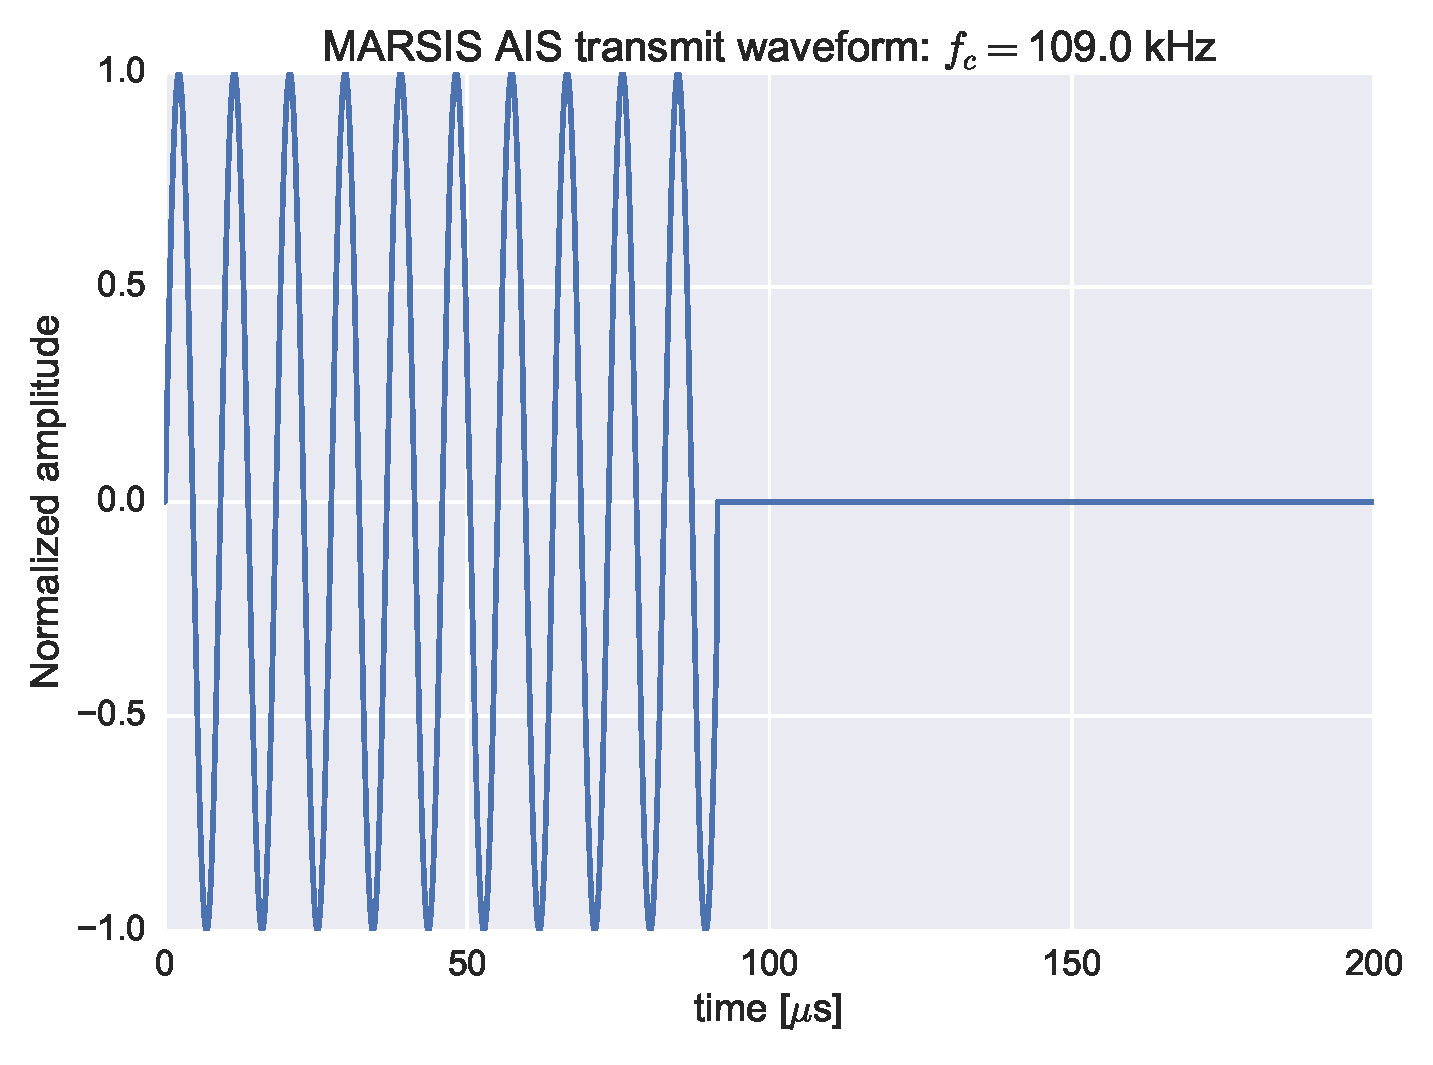
\includegraphics[width=\linewidth]{gfx/marsis_ais_wvfm}
        \caption{Simulated pulse envelope for MARSIS AIS transmission.}		
    \end{subfigure}
    \begin{subfigure}[t]{0.45\linewidth}\centering
        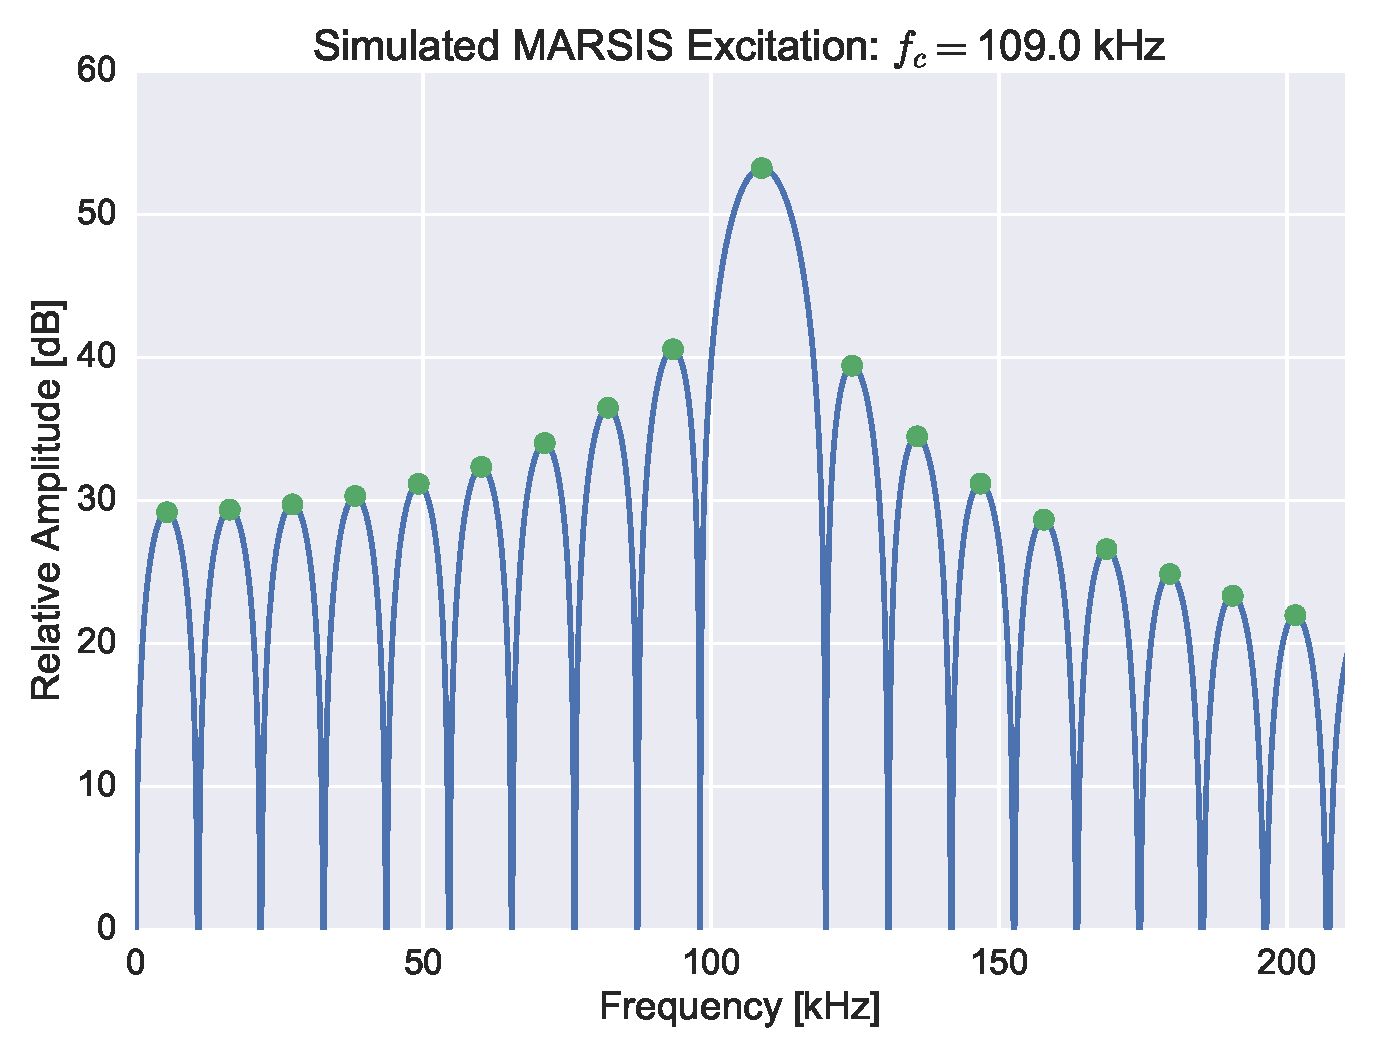
\includegraphics[width=\linewidth]{gfx/marsis_ais_spec}
        \caption{Simulated spectrum for MARSIS AIS transmission.}		
    \end{subfigure}
    \caption{Simulated MARSIS AIS waveform characteristics.}\label{fig:marsispulse}
\end{figure}
Although the radiation efficiency of a \unit[40]{m} dipole is poor for $f_{radar} \ll \unit[1]{MHz}$ the \unit[400]{V} potential on the antenna is quite adequate to simulate local plasma waves \citep{morgan2013}.

The importance of being able to reliably segment HF radar data from the MARSIS instrument is an essential component in assessing over a decade of ionograms from MARSIS. 
Once we are able to reliably segment the foreground ionospheric returns from the many noise sources in the radar data, we can then apply further CV algorithms to extract scientifically relevant parameters in an automated fashion.
Before this and similar independent efforts were undertaken, research groups around the world were typically manually slogging through several weeks of data. 
Most examinations were taking place by clicking and dragging and counting pixels manually \citep{andrews2013,morgan2013}. 

\subsection{Computer Vision background}
Numerous methods of target discrimination have been implemented by radar researchers, including GMM \citep{li2011gmm}.
Several alternate methods for segmenting noisy radar data via background subtraction (BGS) are listed in Table \ref{tab:PrevMeth}. 
\begin{table}\footnotesize	\centering
\caption{Advantage and Disadvantages of Selected BGS methods}\label{tab:PrevMeth}
\begin{tabular*}{1\textwidth}{p{0.3\linewidth}p{0.3\linewidth}p{0.33\linewidth}}
		\toprule
		BGS Method & Advantages & Disadvantages\\
		\midrule
		Per-pixel Moving Average & Simplicity \& speed of computation & Not robust to slow moving objects and/or bimodal backgrounds. Slow adaptation to scene lighting changes. Single, predetermined threshold. \\
		Per-pixel Kalman Filter \citep{ridder1995,koller1994a,koller1994b} & Increased robustness to scene lighting changes, per-pixel automatic threshold & Slow recovery $\Rightarrow$ not robust to bimodal backgrounds \\
		Per-pixel Unimodal Gaussian \citep{pfinder1997} & Advanced multi-class Gaussian ``blob'' foreground models group pixel behavior & Single background mode perhaps best suited for indoor situations\\
		Per-pixel Expectation Maximization (EM) \citep{friedman1997} & Multi-mode learning classification, without operator intervention, auto-tunes parameters over time & Does not forget out-of-date history fast enough. \\
		GMM & Multi-modal background and foreground, robust for: scene lighting changes, repetitive motions, tracking in clutter, slow-moving objects, removed or introduced objects. & Forgets out-of-date history slowly (exponential decay), does not always handle non-Gaussian noises well\\
		\bottomrule
\end{tabular*}
\end{table}
As an additional reference point, a static intensity threshold was implemented with the results shown in section~\ref{sec:ApxSeg}.
It was apparent from this initial effort that more than Otsu thresholding \citep{otsu1979} or multilevel thresholding \citep{huang2011} was needed, leading to the successful implementation of GMM for ionospheric target discrimination.

\FloatBarrier
\subsection{Segmentation by Static Intensity Threshold}\label{sec:ApxSeg}
One example of a basic segmentation technique is using a static intensity threshold on an image to segment foreground from background pixels. 
Although this method is not of the same class as GMM segmentation, static thresholding is briefly shown on the MARSIS data to show that the MARSIS segmentation problem is not trivially simple. 
The first step in designing the static threshold is examining the histogram of the image data and determining an intensity threshold that divides foreground pixels from presumably weaker (in intensity) background pixels. 
Consider the example in Figure~\ref{fig:rawImg}, with normalized histogram in Figure~\ref{fig:rawHist}. 
As a first try for this MARSIS data, based on Figure~\ref{fig:rawHist}, we declare all pixels with intensity $I\geq10^{-15}$ to be foreground, and all pixels with $I<10^{-15}$ to be background. 
This segmentation by static intensity threshold results in the thresholded intensity output of Figure~\ref{fig:bwTseg} with the new normalized histogram of Figure~\ref{fig:bwThist}. 
The limited dynamic range of the thresholded intensity data appears nearly like a binary image. 
Manual inspection of the remaining pixel values in Figure~\ref{fig:bwTseg} showed that the non-ionosphere pixels are of equal or greater intensity than the ionospheric pixels, so static threshold segmentation alone was not sufficient for MARSIS data segmentation.

\begin{figure}
	\begin{minipage}[b]{0.5\linewidth} %<-- [b] makes both figures be bottom-aligned (looks a lot better)
		\centering %<-- use this instead of \begin{center}
		\includegraphics[trim=65 580 320 75,clip,width=1\linewidth]{gfx/SimpleThres}
		\caption{Raw MARSIS Intensity Data}\label{fig:rawImg}
	\end{minipage}
	\begin{minipage}[b]{0.5\linewidth}
		\centering
		\includegraphics[trim=300 530 45 40,clip,width=1\linewidth]{gfx/SimpleThres}
		\caption{Raw MARSIS Intensity Histogram}\label{fig:rawHist}
	\end{minipage}
\end{figure}

\begin{figure}
	\begin{minipage}[b]{0.5\linewidth}
		\centering
		\includegraphics[trim=65 330 320 275,clip,width=1\linewidth]{gfx/SimpleThres}
		\caption{Image after Thresholding} \label{fig:bwTseg}
	\end{minipage}
	\begin{minipage}[b]{0.5\linewidth}
		\centering
		\includegraphics[trim=300 295 45 275,clip,width=1\linewidth]{gfx/SimpleThres}
		\caption{Normalized Histogram of thresholded intensity data}\label{fig:bwThist}
	\end{minipage}
\end{figure}

\FloatBarrier
\subsection{Non-GMM methods}
\subsubsection{Per-Pixel Moving Average}
A background image $B$ may be constructed of the long-term average from each pixel intensity at $I(x,y,t)$ incrementally \citep{friedman1997} by 
\begin{equation} \label{eq:RolAvg}
B(x,y,t) = \frac{t-1}{t}B(x,y,t-1)+\frac{1}{t}I(x,y,t).
\end{equation}
By inspection of \eqref{eq:RolAvg}, it is apparent that long-ago pixels will still play a too-significant role in the current background image.
Adding a ``forgetting factor'' \citep{friedman1997} 
\begin{equation}\label{eq:forgetRol}
B(x,y,t)=(1-\alpha)B(x,y,t-1)+\alpha I(x,y,t)
\end{equation}  
will make old pixels have an exponential weighting decay, thereby increasing the relevance of more recent pixels. 
It appears that the moving average assumes that a single background model is sufficient at any given time, but such a model is likely to fail in bimodal backgrounds such as static crashes in a radar receiver, or the significantly changing return signal strength versus distance to target and plasma density. 
Thus, the moving average technique was deemed inadequate for the MARSIS work.

\FloatBarrier
\subsubsection{Per-pixel Kalman Filter}
The per-pixel Kalman filter BGS technique has seen many variations by workers since the 1990s, including \citet{ridder1995,koller1994a,koller1994b}.
A typical implementation uses matched linear filters, with \textit{a priori} knowledge of the intensities of desired foreground and unwanted background pixels. 
In situations where the background noise intensity may exceed the actual foreground intensity, and the background noise is highly spatiotemporally dynamic, members of the family of Kalman filtering techniques may incorrectly label excessive proportions of background pixels erroneously as foreground pixels. 
Also, if the background pixels have similar amplitude trends, i.e., the background pixels have non-zero correlation with the foreground pixels, Kalman filtering may incorrectly classify background and foreground pixels in the same class.
Highly dynamic background scenes (such as are common in HF radar) require a model that can adapt quickly, discarding irrelevant background models for new models constantly during the real-time video tracking process.

\FloatBarrier
\subsubsection{Per-pixel Unimodal Gaussian}
The per-pixel unimodal Gaussian BGS technique \citep{pfinder1997} is updated on a per-pixel basis by $\mu_t=(1-\alpha)\mu_{t-1} + \alpha X_t$, where $X_t$ is the value of the latest pixel and $\alpha$ is a user selected learning-rate parameter. This is the same method used to update the mean in GMM in \eqref{eq:muUpdate}. Unlike GMM, there is no discarding of stale background information as spatiotemporal dynamics potentially make many background pixels appear as foreground.
This method therefore has too simple a background model for dynamic HF radar applications, unlike GMM.

\FloatBarrier
\subsubsection{Per-pixel Expectation Maximization}
One of the key weaknesses of EM BGS, as acknowledged by the authors themselves \citep{friedman1997}, is that the algorithm must be primed with \textit{a priori} information about expected pixel intensity vs. classification. 
The mixture model is updated over time, but could be mislead by rapid fluctuations to mis-classify foreground as background and vice-versa.
Rather than being stuck rigidly to three types of possibly erroneous classifications, GMM allows classifications to be fluid as the situation dynamics demand, to be described in section \ref{sec:GMMadv}.

\subsection{Advantages of Proposed Method} \label{sec:GMMadv}
One of the key advantages of GMM as put forth by \citet{stauffer1999} are that it can handle highly spatiotemporally dynamic backgrounds, without a need for \textit{a priori} foreground and background parameters. 
The GMM algorithm is computationally tractable for on-line implementation with modest computational resources.
GMM can have arbitrary proportions of the distributions as foreground or background, versus other algorithms that have \textit{fixed} proportions of the distributions assigned to foreground and background. 

For the HF radar data, intensity of all pixels varies over several orders of magnitude across only several frames of data.
An intensity distribution that ten frames ago corresponded to ``background'' may now be ``foreground,'' and so a suitable BGS algorithm must be able to quickly assign distributions to foreground or background in the proportions suitable for the dataset. 
Because GMM requires consistent evidence over time of a pixel belonging to a distribution for that distribution's weight to be increased, GMM is not excessively sensitive to transients of any spatial extent. 
Repetitive behaviors are learned and classified as background as well as typical radar noise and interference. 

\FloatBarrier
\subsection{GMM Technical Summary}\label{sec:TechSum}
A block diagram of the GMM algorithm is depicted in Figure \ref{fig:gmmbasic}. 
\begin{figure}\centering
	\includegraphics[width=0.6\linewidth]{gfx/GMMflowchart}
	\caption{GMM flowchart for each pixel, each frame.}\label{fig:gmmbasic}
\end{figure}
Under GMM, the probability of observing a pixel value at time $t$ is given by \begin{equation}\label{eq:totProb}
P\left(X_t\right)=\sum_{i=1}^K\omega_{i,t}\cdot\mathcal{N}\left(X_t,\mu_{i,t},\Sigma_{i,t}\right)
\end{equation}
where $\omega_{i,t}$ is the current weight for the $i^{th}$ Gaussian distribution model (GDM), $\mu_{i,t}$ is the current mean of the $i^{th}$ GDM, and $\Sigma_{i,t}$ is the covariance matrix of the $i^{th}$ GDM. 
Each GDM $\mathcal{N}$ is represented by
\begin{equation}\label{eq:GDM}
\mathcal{N}\left(X_t,\mu,\Sigma\right)=\frac{1}{(2\pi)^\frac{1}{2}\left|\Sigma\right|^\frac{1}{2}}\text{Exp}\left[-\frac{1}{2}\left(X_t-\mu_t\right)^T\Sigma^{-1}\left(X_t-\mu_t\right)\right].
\end{equation} 
In the application to MARSIS data, the covariance matrix is
\begin{equation}
\Sigma_{k,t}\equiv\sigma_k^2.
\end{equation} 

First, the new pixel $X_t$ is checked for a match to existing distributions by
\begin{equation} \label{eq:gotMatch}
\begin{cases}
|X_t-\mu_k| \leq 2.5\sigma_k    & k^{th}\text{-distribution is ``match''$\Rightarrow$ Do algorithm A}  \\
|X_t-\mu_k| > 2.5\sigma_k & k^{th}\text{-distribution is non-matching $\Rightarrow$ Do algorithm B}
\end{cases}
\end{equation}

\subsubsection{GMM Algorithm A} 
GMM Algorithm A applies only when $X_t$ has a ``match''. 
The steps of Algorithm A repeat for each pixel in the current frame--in a system capable of parallel processing, such as an FPGA or multi-core CPU, Algorithm A may be executed in parallel for each pixel in a frame, potentially giving a great processing speed up.
\begin{enumerate}
	\item Update all distribution weights by 
	\begin{equation} \label{eq:weightUpdate}
	\omega_{k,t}=(1-\alpha)\omega_{k,t-1}+\alpha(M_{k,t})
	\end{equation}	
	\begin{equation} \label{eq:meq}
	M_{k,t} =
	\begin{cases}
	1 & \text{if model matched pixel}  \\
	0 & \text{if model did not match pixel} 
	\end{cases}
	\end{equation}
	
	\item Update $\mu_k$ and $\sigma_k$ of model which ``matched'' by 
	\begin{equation} \label{eq:muUpdate}
	\begin{split}
	\mu_t      & =(1-\rho)\mu_{t-1}+\rho X_t \\
	\sigma^2_t & =(1-\rho)\sigma^2_{t-1}+\rho(X_t-\mu_t)^T(X_t-\mu_t) \\
	\rho	   & =\alpha\mathcal{N}(X_t|\mu_k,\sigma_k)
	\end{split}
	\end{equation}
	
	\item In descending order, sort distributions by ``fitness'' $\frac{\omega_k}{\sigma_k}$
	
	\item Take cumulative sum of sorted weights $\omega_k$ until threshold is reached as in 
	\begin{equation} \label{eq:compSum}
	B = \argmin\limits_k \left(\sum_{k=1}^{b}\omega_k>T\right).
	\end{equation}
	Only distribution models with weights included in \eqref{eq:compSum} below threshold $T$ are declared ``background.''
	
	\item If $X_t$ matched a distribution included in the background model $B$, $X_t$ is classified as a \textbf{background pixel}. Else, $X_t$ is classified as a \textbf{foreground pixel}.
\end{enumerate}

\FloatBarrier
\subsubsection{GMM Algorithm B}
GMM Algorithm B applies only when $X_t$ does \textit{not} have a matching distribution model. 
Like GMM Algorithm A, the steps of GMM Algorithm B repeat for each pixel in the current frame, and may likewise be executed in parallel on a capable system.
\begin{enumerate}
	\item Discard distribution model with lowest weight (that is, model least corresponding to trending pixel data) $\omega_{k,min}=\argmin\limits_k\left(\omega_k\right)$.
	\item Create a replacement distribution ``r'' with weight $\omega_{r}=\omega_{k,min}$, mean $\mu_r=\mu_{k,min}$, and a higher variance using: $\sigma_r=2.5\cdot\sigma_{k,min}$
	\item $X_t$ is classified as a \textbf{foreground} pixel.
\end{enumerate}

\FloatBarrier
\subsection{GMM-based algorithm parameters for MARSIS data}
An essential part of the computer vision algorithm design process is scrutinizing the statistics of the relevant processes. 
Figure~\ref{fig:bighisto} shows histograms selected from data available across the entire MARSIS operating period. 
\begin{sidewaysfigure}
	\centering
	\includegraphics[trim=5 220 15 30,clip,width=.95\linewidth]{gfx/Histo}
	\caption{Histograms of Selected MARSIS Orbits}\label{fig:bighisto}
\end{sidewaysfigure}
Daily Sunspot data was obtained from SIDC \citet{sidc}, plotted across the time range of MARSIS data in Figure \ref{fig:sunspots}.
\begin{figure}
	\centering
	\includegraphics[trim=50 40 50 70,clip,width=.5\linewidth]{gfx/Sunspots}
	\caption{Sunspots: Solar Cycle 23--24, Years 2005-2011}\label{fig:sunspots}
\end{figure} 
The sunspot count (sunspot number) is relevant to MARSIS data since sunspot number is correlated with solar flux and coronal mass ejection (CME) events \citep{webb1994} that drive ionospheric processes of interest at Mars.
A potential computer vision algorithm pitfall is developing an algorithm that works for a given data set or subset of a larger family of data, but that will not handle all necessary data. 

We observe from the histograms in Figure~\ref{fig:bighisto} that there appear to be at least three statistical distributions active in the data.
From manual inspection of several orbital data sets, one or two distributions attributable to noises of \#6 and \#7 from Table~\ref{tab:sigCat} are evident in Figure~\ref{fig:bighisto} with mean intensities near $10^{-23}$, and in any case the means of these noises are observed to be less than $10^{-20}$. 
GMM will automatically learn how many distributions should be attributed to background, but we do want to choose an appropriate total number of distributions $K$, since too-large $K$ will results in needless computational expense, while too-small $K$ will result potential GMM breakdown as the distributions cannot be assigned consistently.

\section{Experiments}
\subsection{Experimental Data}
The MARSIS data used in this project was arbitrarily sampled from the years 2005--2011. 
The primary driving force behind the photochemical processes in the ionosphere is the Sun, which goes through eleven-year solar cycles. 
The number of sunspots is generally proportional to the intensity of the solar energy impinging upon the Martian ionosphere. 
A plot of the observed daily sunspot number with the orbits selected is depicted in Figure \ref{fig:sunspots}.
The red line portions are times over which MARSIS data is not available, while blue line time segments are times where MARSIS data is available.

\subsection{Experimental Results}
The \citet{cvmarsis} implementation executes the steps shown in section~\label{TechSum}. 
An example frame of MARSIS data is shown in Figure~\ref{fig:rawImg}, while the learning data is shown in Figure~\ref{fig:learnData}.  
\begin{figure}	\centering
	\includegraphics[trim=0 0 0 50,clip,width=\textwidth]{gfx/2107_22MHz}
	\caption{GMM Learning Data on a Single Pixel}\label{fig:learnData}
\end{figure}
The basic steps of the \citet{cvmarsis} algorithm over and above the previously discussed steps are as follows:
\begin{enumerate}
	\item Load most recent frame of image data
	\item Compute mean $\mu_{t-1}$ and standard deviation $\sigma_{t-1}$ using entire image frame
	
	\item Create starting $\mu$ and $\sigma$ by multiplying by $K$ arbitrary constants. We chose to use the constants: $\{ 0.1,0.25,0.5,1.0,2.0\}$, and so: \\
	
	$\mu_{k,t-1}=\{ 0.1,0.25,0.5,1.0,2.0\}\cdot\mu_{t-1}$ \\
	$\sigma_{k,t-1}=\{0.1,0.25,0.5,1.0,2.0\}\cdot\sigma_{t-1}$
	
	\item The weights for each Gaussian distribution are initialized to all be equal, that is:
	\[
	\omega_{k,t-1}=\frac{1}{K}
	\]
	\item Run GMM algorithm 
	\item Execute connected components algorithm on entire frame of data
	\item Execute tracking algorithm on sequential frames of data
\end{enumerate}


\section{Conclusions}
The GMM algorithm described by \citet{stauffer1999,kaew2001} and implemented for MARSIS data in \citet{cvmarsis} has been shown to be useful as applied to the challenging MARSIS background subtraction problem. 
This algorithm helped influence not only existing MARSIS global analysis trends but has been extended to passive radar in chapter~\ref{chapter:passive}. 
GMM have been shown to be computationally tractable for real-time data as well as off-line analysis of recorded data. 
The ability of GMM to cope with large, regular changes in the statistics of the background leads to a wide range of useful applications of GMM.

While there is no one perfect solution for the wide variety of background segmentation tasks, for MARSIS, GMM has been shown to be a strong candidate to consider for BGS tasks. 
Although GMM can be fooled for pixels close in intensity and spatiotemporal behavior of the ground truth foreground, these isolated pixels could be removed by post-segmentation computer vision algorithms. 
MATLAB includes GMM algorithms in a toolbox based on GMM and subsequent refinements, which lends credence to the usefulness of GMM to a variety of problems. 
